%%%%%%%%%%%%%%%%%%%%%%%%%%%%%%%%%%%%%%%%%%%%%%%%%%%%%%%
%                   File: OSAmeetings.tex             %
%                  Date: March 21, 2007  MSD          %
%                                                     %
%     For preparing LaTeX manuscripts for submission  %
%       submission to OSA meetings and conferences    %
%                                                     %
%       (c) 2007 Optical Society of America           %
%%%%%%%%%%%%%%%%%%%%%%%%%%%%%%%%%%%%%%%%%%%%%%%%%%%%%%%

\documentclass[letterpaper,10pt]{article}
\usepackage{osameet2}

%% standard packages and arguments should be modified as needed

\usepackage{amsmath,amssymb}
\usepackage{floatrow}
\usepackage[export]{adjustbox}

% \bibliography{paper}
% \bibliographystyle{osajnl}


%\usepackage[pdftex,colorlinks=true,bookmarks=false,citecolor=blue,urlcolor=blue]{hyperref} %pdflatex
\usepackage[colorlinks=true,bookmarks=false,citecolor=blue,urlcolor=blue]{hyperref} %latex w/dvips


\begin{document}

\title{Three-Dimensional Fluorophore Orientation Imaging with Multiview Polarized Microscopy}

\author{Talon Chandler,${}^{1,*}$ Min Guo,${}^2$ Shalin Mehta,${}^{1,3,4}$ Abhishek Kumar,${}^2$\\ Hari Shroff,${}^{2,5}$ Rudolf Oldenbourg,${}^{3,6}$ Patrick J. La Rivi\`ere${}^{1,5}$}

\address{${}^1$Department of Radiology, University of Chicago, Chicago, Illinois 60637, USA.\\ ${}^2$Section on High Resolution Optical Imaging, National Institute of Biomedical Imaging\\ and Bioengineering, National Institutes of Health, Bethesda, Maryland 20892, USA.\\ ${}^3$Bell Center, Marine Biological Laboratory, Woods Hole, Massachusetts 02543, USA.\\ ${}^4$(present address) Chan Zuckerberg Biohub, San Francisco, California 94158, USA.\\ ${}^5$Whitman Center, Marine Biological Laboratory, Woods Hole, Massachusetts 02543, USA.\\ ${}^6$Department of Physics, Brown University, Providence, Rhode Island 02912, USA.}
\email{${}^*$talonchandler@talonchandler.com} %% email address is required

\begin{abstract}
  \hspace{-0.75em} We show that polarized fluorescence microscopes make
  band-limited measurements in the angular frequency domain. We use this result
  to propose and demonstrate efficient algorithms for reconstructing
  three-dimensional fluorophore orientations from multiview polarized microscope
  data.
\end{abstract}
\vspace{0.03em}
\ocis{180.2520 Fluorescence microscopy, 260.5430 Polarization}
\vspace{-1em}
\section{Introduction}
Polarized fluorescence microscopes can measure the orientation of fluorophores
in live specimens\cite{weiss1999}. Unfortunately, existing techniques are
limited to imaging two-dimensional orientations, and attempts to generalize
these approaches to three-dimensional orientations have faced computational
difficulties. We propose the use of the spherical harmonics to simplify the
analysis of polarized fluorescence microscopes. In the same way that the Fourier
transform simplifies the analysis of spatial imaging systems, the spherical
Fourier transform simplifies the analysis of angular imaging systems.

\section{Theory}
Consider a small voxel that contains many non-interacting fluorophores. We define the
orientation distribution function $f(\hat{\mathbf{s}})$ as the number of
fluorophores per steradian oriented in a direction $\hat{\mathbf{s}}$. The goal
of polarized fluorescence microscopy is to estimate $f(\hat{\mathbf{s}})$ in
many voxels throughout a three-dimensional sample.

The forward model for an $N$-measurement polarized fluorescence microscope is
given by
\begin{align}
  g_i = \int_{\mathbb{S}^2}d\hat{\mathbf{s}}\ h_i(\hat{\mathbf{s}})f(\hat{\mathbf{s}})\hspace{1em}\text{for}\hspace{1em} i=1,\dotsc,N,
\end{align}
where $h_i(\hat{\mathbf{s}})$ is the kernel of the $i$th microscope
configuration, the integral is over the sphere $\mathbb{S}^2$, and $g_i$ is the
$i$th intensity measurement. Note that we are applying this forward model to
each voxel independently---we assume that there is no spatial blurring so the
signal from each voxel is independent. By discretizing $f(\hat{\mathbf{s}})$ and
expanding $h(\hat{\mathbf{s}})$ in terms of the spherical harmonics, we can
rewrite Eq. (1) as
\begin{align}
  \mathbf{g} = \Psi\hspace{0.1em}\mathbf{B}^+\mathbf{f},
\end{align}
where $\mathbf{f} = [f(\hat{\mathbf{s}}_1), \cdots, f(\hat{\mathbf{s}}_R)]^T$ is
a vector of $R$ samples of $f(\hat{\mathbf{s}})$; $\mathbf{B}$ is a matrix of
the spherical harmonics evaluated at the sample points,
$\mathbf{B}_{ij} = Y_j(\hat{\mathbf{s}}_i)$ where $Y_j$ is the $j$th spherical
harmonic; $\cdot^+$ is the Moore-Penrose pseudoinverse; $\Psi$ is a matrix of
the spherical harmonic coefficients of the kernels,
$\Psi_{ij} = \int_{\mathbb{S}^2}d\hat{\textbf{s}}\
h_i(\hat{\mathbf{s}})Y_j(\hat{\mathbf{s}})$; and
$\mathbf{g} = [g_1, \cdots, g_N]^T$ is a vector of the $N$ intensity
measurements.

The kernels for a wide class of polarized fluorescence microscopes have been
calculated previously\cite{chandler}. For many polarized fluorescence
microscopes the kernel can be expanded in terms of a small number of spherical
harmonics. If the kernel can be expanded in terms of $M$ spherical harmonics
then $\Psi$ is an $N\times M$ matrix and $\mathbf{B}^+$ only needs to be
calculated in the first $M$ columns. This simplification reduces Eq. (1) from
a set of integrals to an efficient series of matrix multiplications.

\section{Methods and Results}
We labeled the actin filaments of a fixed-cell sample with Alexa Fluor 488
Phalloidin and imaged the sample with an asymmetric 1.1/0.71 NA dual-view
inverted selective plane illumination microscope with orthogonal objectives
\cite{wu2017} and variable polarizers added to both illumination paths. The
dipole moment of Alexa Fluor 488 Phalloidin is known to align parallel to the
long axis of actin filaments, so this sample makes a suitable test specimen for
our reconstruction algorithm. We imaged the specimen volume eight times---two
views with four illumination polarization orientations each.

To reconstruct the orientation in each voxel we solved the following problem 
\begin{align}
\mathbf{f^{\thinspace *}}= \underset{\mathbf{f}\in\{\mathbf{e}_i\}\ i = 0,\dotsc,R}{\text{argmin}}
\ \ ||\thinspace\mathbf{g} - \Psi\hspace{0.1em}\mathbf{B}^+\mathbf{f}\thinspace||_2^2,
\end{align}
where $\mathbf{e}_i$ is a vector with a one in the $i$th entry and zeros
elsewhere. By constraining $\mathbf{f}$ we are assuming that all of the
fluorophores in each voxel are oriented in the same direction---a reasonable
assumption for this sample.
\begin{figure}[htbp]
  \centering
  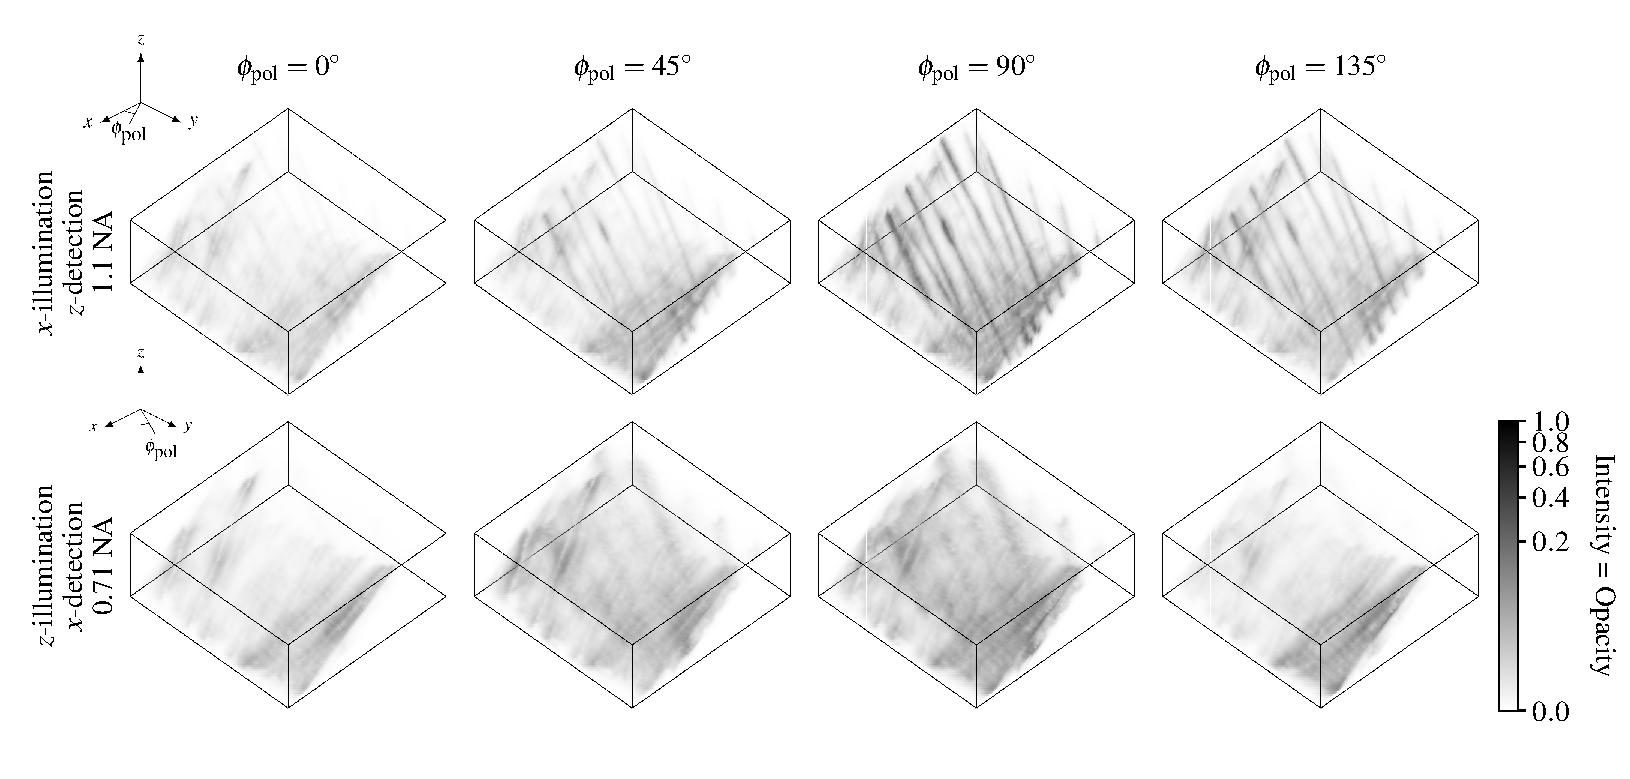
\includegraphics[width=16.cm, trim={0.1cm 1.3cm 0 0.5cm}]{figs/roi2/data.pdf}
  \caption{Fluorescence intensities of a small volume
    ($13.5\times 13.5\times 5.4\ \mu$m${}^3$) of a cell that was fixed, stained
    with Alexa Fluor 488 Phalloidin, and imaged in a dual-view microscope
    (diSPIM). The staining reveals two sets of actin bundles. Because
    fluorophores are aligned parallel to the bundles, their fluorescence
    intensities are modulated by the propagation direction and polarization of
    the excitation light. Bundles from bottom right to top left are highlighted
    for $x$-illumination and $z$-detection with
    $\phi_{\text{pol}} = 90^{\circ}$, while their intensities almost disappear
    for $z$-illumination and $x$-detection with $\phi_{\text{pol}} = 0^{\circ}$,
    which reveals the bundles running from bottom left to top right.}
\end{figure}

\begin{minipage}{.263\textwidth}
  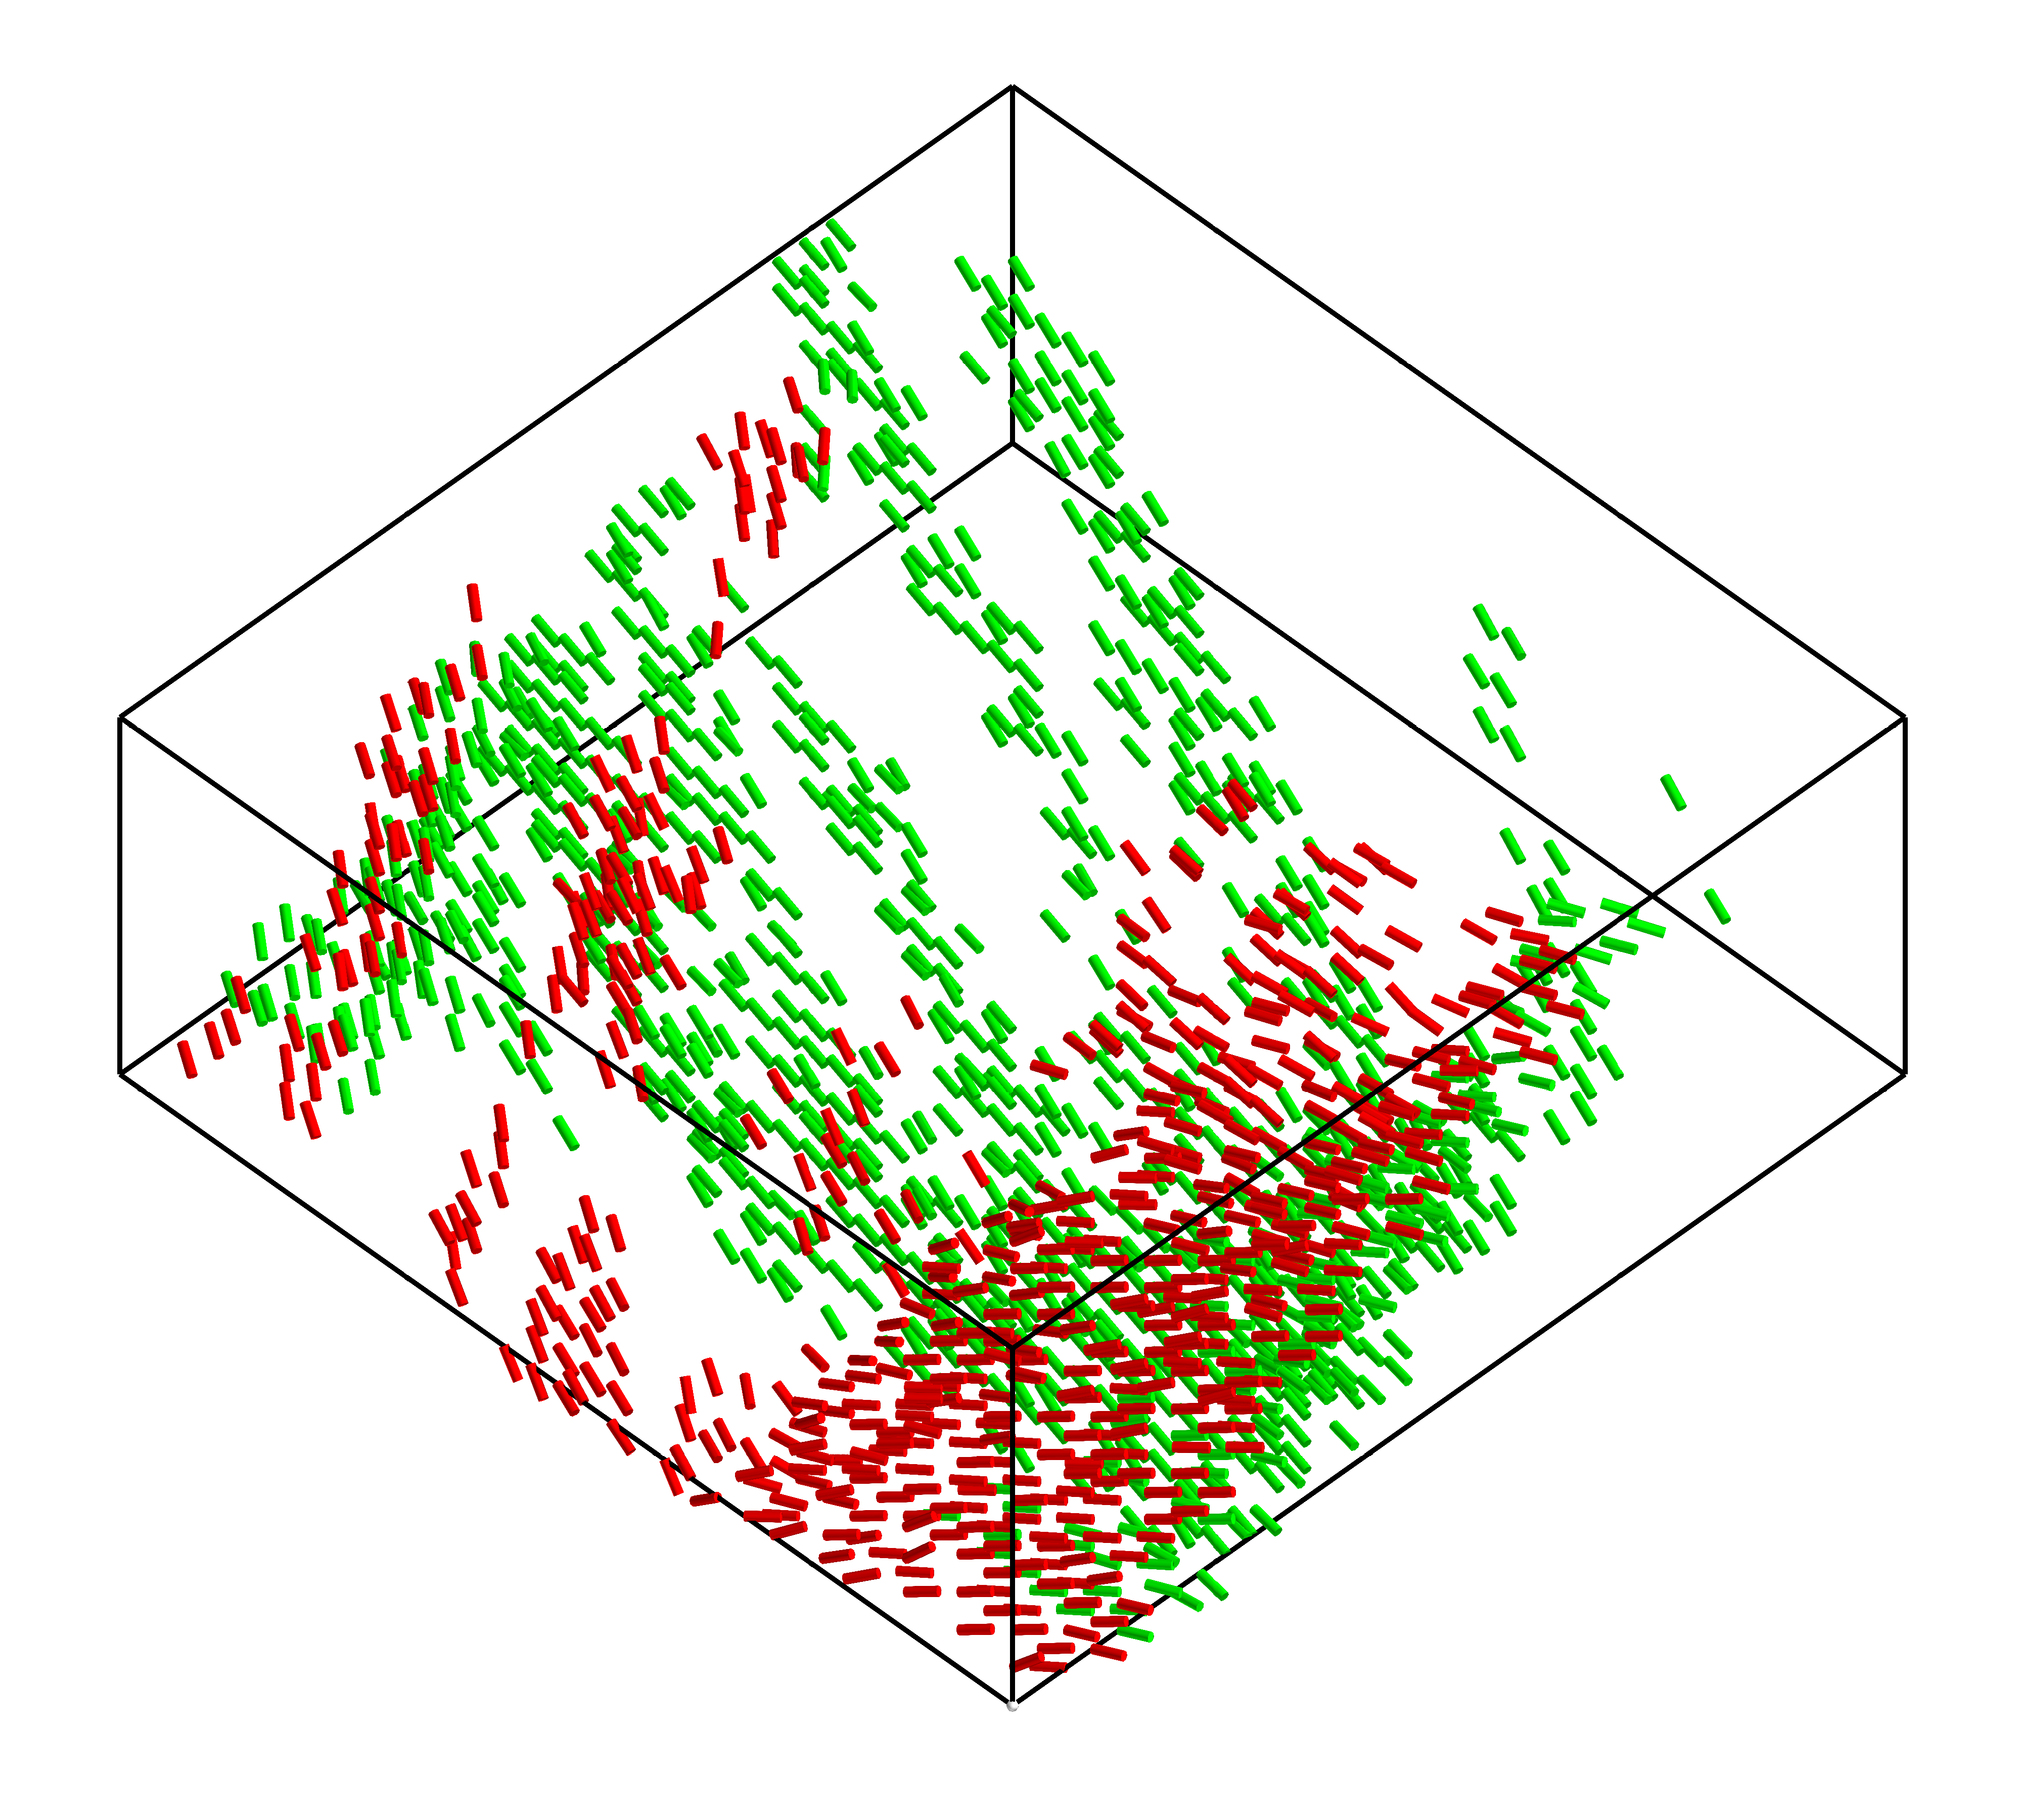
\includegraphics[width=3.7cm, trim={0cm 0cm 0 0cm}, right]{figs/roi2/recon_color-min.png}
\end{minipage}% This must go next to `\end{minipage}`
\begin{minipage}{.639\textwidth}
  Fig. 2. Reconstruction of fluorophore orientations based on all intensity
    data shown in Fig. 1. Orientations are shown as short lines only in voxels
    whose fluorescence intensities surpassed a threshold. To highlight the two
    sets of actin bundles discussed in the caption of Fig. 1, we split the
    volume with a plane and colored the proximal voxels red and the distal
    voxels green. The reconstructed orientations approximately align with the
    long axes of the actin filaments as expected.
\end{minipage}
 \vspace{-1em}
{\footnotesize\bibliography{abstract}{}}
\bibliographystyle{osajnl}

\end{document}
